% !TeX document-id = {c68f4be8-c497-43e0-82df-e9ebfbea9577}
% !TeX TXS-program:pdflatex = pdflatex -synctex=1 -interaction=nonstopmode --shell-escape %.tex
% новая команда \RNumb для вывода римских цифр
\documentclass[a4paper,12pt]{article}
\usepackage{amssymb}
\usepackage{amsmath}
\usepackage{amsthm} 
\usepackage{caption}
\usepackage{misccorr}
\usepackage[noadjust]{cite}
\usepackage{cmap} 
\usepackage[utf8]{inputenc}
\usepackage[T2A]{fontenc}
\usepackage[english, russian]{babel}
\usepackage{graphics}
\usepackage{graphicx}
\usepackage{textcomp}
\usepackage{verbatim}
\usepackage{makeidx}
\usepackage{geometry}
\usepackage{float}
\usepackage{bm}
\usepackage{esint}
\usepackage{mathtools}
\usepackage{graphicx}
\usepackage{listings}
\usepackage{courier}
\usepackage{multirow}
\usepackage{graphicx}
\usepackage[table]{xcolor}
\usepackage{color}
\usepackage[most]{tcolorbox} 
\usepackage{diagbox}

\lstset{basicstyle=\fontsize{10}{10}\selectfont,breaklines=true}

\newcommand{\specchapter}[1]{\chapter*{#1}\addcontentsline{toc}{chapter}{#1}}
\newcommand{\specsection}[1]{\section*{#1}\addcontentsline{toc}{section}{#1}}
\newcommand{\specsubsection}[1]{\subsection*{#1}\addcontentsline{toc}{subsection}{#1}}
\newcommand{\RNumb}[1]{\uppercase\expandafter{\romannumeral #1\relax}}
\newcommand{\jj}{\righthyphenmin=20 \justifying}


% геометрия
\geometry{pdftex, left = 2cm, right = 2cm, top = 2.5cm, bottom = 2.5cm}

\setcounter{tocdepth}{4} % фикс переноса 
\righthyphenmin = 2
\tolerance = 2048

\begin{document}
\thispagestyle{empty}

\noindent \begin{minipage}{0.15\textwidth}
	
\includegraphics[width=\linewidth]{b_logo}
\end{minipage}
\noindent\begin{minipage}{0.9\textwidth}\centering
	\textbf{Министерство науки и высшего образования Российской Федерации}\\
	\textbf{Федеральное государственное бюджетное образовательное учреждение высшего образования}\\
	\textbf{«Московский государственный технический университет имени Н.Э.~Баумана}\\
	\textbf{(национальный исследовательский университет)»}\\
	\textbf{(МГТУ им. Н.Э.~Баумана)}
\end{minipage}

\noindent\rule{18cm}{3pt}
\newline\newline
\noindent ФАКУЛЬТЕТ $\underline{\text{«Информатика и системы управления»}}$ \newline\newline
\noindent КАФЕДРА $\underline{\text{«Компьютерные системы и сети»}}$\newline\newline
\noindent НАПРАВЛЕНИЕ ПОДГОТОВКИ $\underline{\text{«09.03.04 Программная инженерия»}}$\newline\newline\newline\newline\newline


\begin{center}
	\noindent\begin{minipage}{1.3\textwidth}\centering
	\Large\textbf{  ОТЧЕТ }\newline
	\textbf{по лабораторной работе №5}\newline\newline
	\end{minipage}
\end{center}

\noindent\textbf{Название:} $\underline{\text{Исследование мультиплексоров}}$\newline\newline
\noindent\textbf{Дисциплина:} $\underline{\text{Архитектура ЭВМ}}$\newline\newline\newline\newline\newline

\begin{center}
	\begin{tabular}{ccccc}
		Студент: & $\underline{\text{ИУ7-43Б}}$ & $\underline{\text{~~~~~~~~~~~}}$ & $\underline{\text{28.04.2020}}$ & $\underline{\text{А. В. Романов}}$ \\
		 & \footnotesize группа & \footnotesize подпись & \footnotesize дата  & \footnotesize (И. О. Фамилия) \\
		  &  &  &  & \\
		Преподаватель: & \textbf{} & $\underline{\text{~~~~~~~~~~~}}$ & $\underline{\text{~~~~~~~~~~~~}}$ & $\underline{\text{А. Ю. Попов}}$ \\
		&  & \footnotesize подпись & \footnotesize дата  & \footnotesize (И. О. Фамилия) \\
	\end{tabular}
\end{center}


\begin{center}
	\vfill
	Москва~---~\the\year
~г.
\end{center}
\clearpage

\section{Цель работы} Изучение принципов построения, практического применения и экспериментального исследования мультиплексоров.

\section{Исследование ИС ADG408 или ADG508 в качестве коммутатора MUX 8 – 1 цифровых сигналов}

\noindent Вариант 18 ($D_{0}...D_{7}$: 01001000)
\begin{center}
	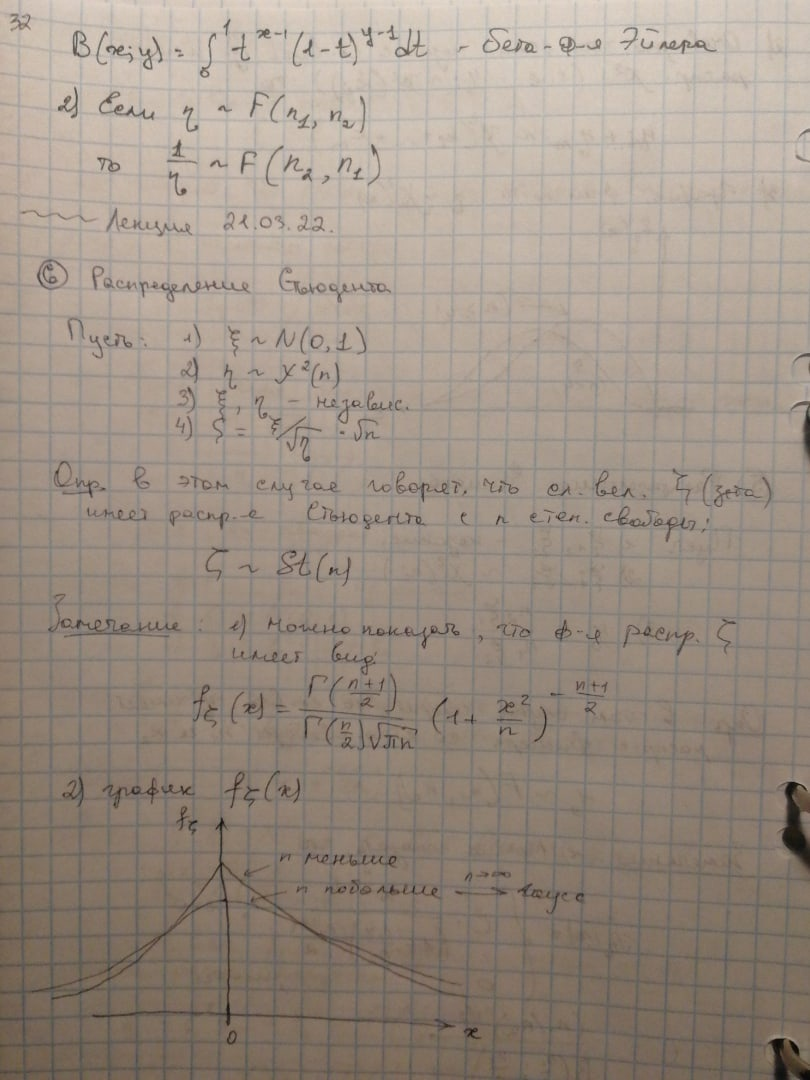
\includegraphics[scale=0.65]{../screens/1.jpg}
	
	""
	
	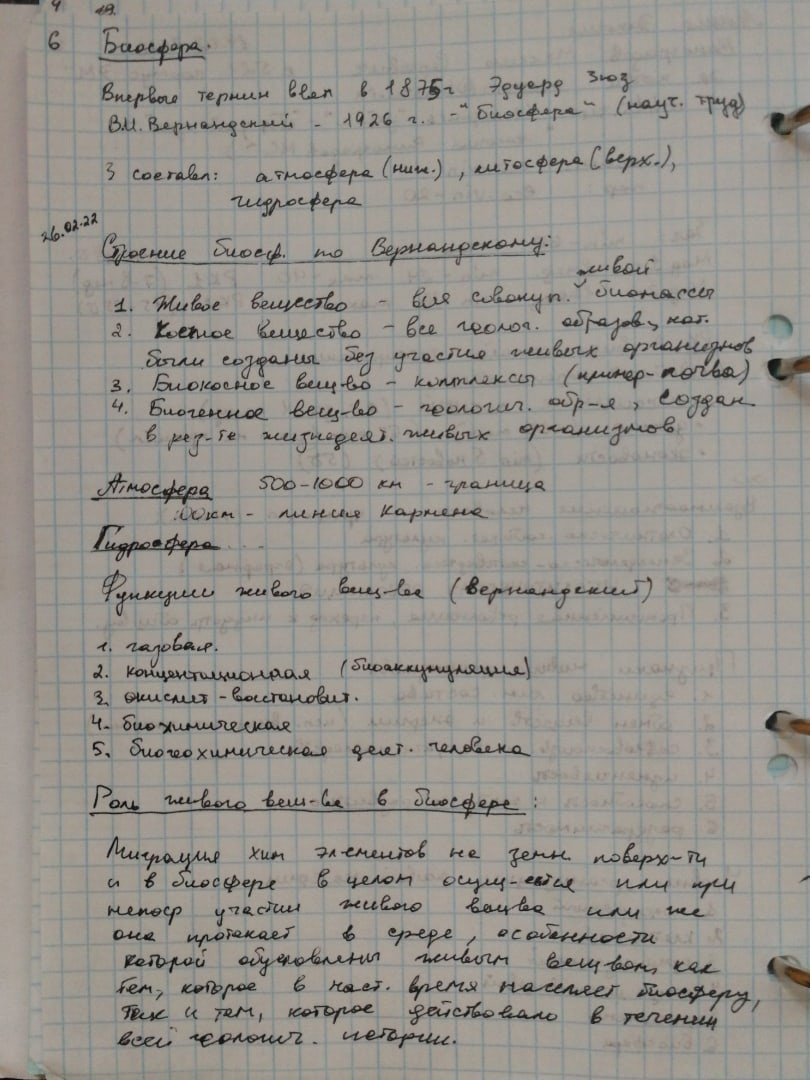
\includegraphics[scale=0.68]{../screens/2.jpg}
\end{center}

\noindent Мультиплексор может быть анализатором логической функции. Изучив сигналы, приходим к выводу что они совпадают с входными данными. \newline

\noindent Файл: 1.ms\newline

\section{Исследование ИС ADG408 или ADG508 в качестве коммутатора MUX 8 – 1 аналоговых сигналов}

\begin{center}
	
\includegraphics[scale=0.7]{../screens/3.jpg}
	
	""
	
	
\includegraphics[scale=0.75]{../screens/4.jpg}
\end{center}

\noindent На мультиплексоре получается получаем истину при достижении напряжения больше чем половина напряжения $EN$.\newline

\noindent Файл: 2.ms

\section{Исследование ИС ADG408 или ADG508 как коммутатора MUX 8 – 1 цифровых сигналов в качестве формирователя ФАЛ четырех переменных}

\noindent Набор значений $D_{0}...D_{7}$: 01110011
\begin{center}
	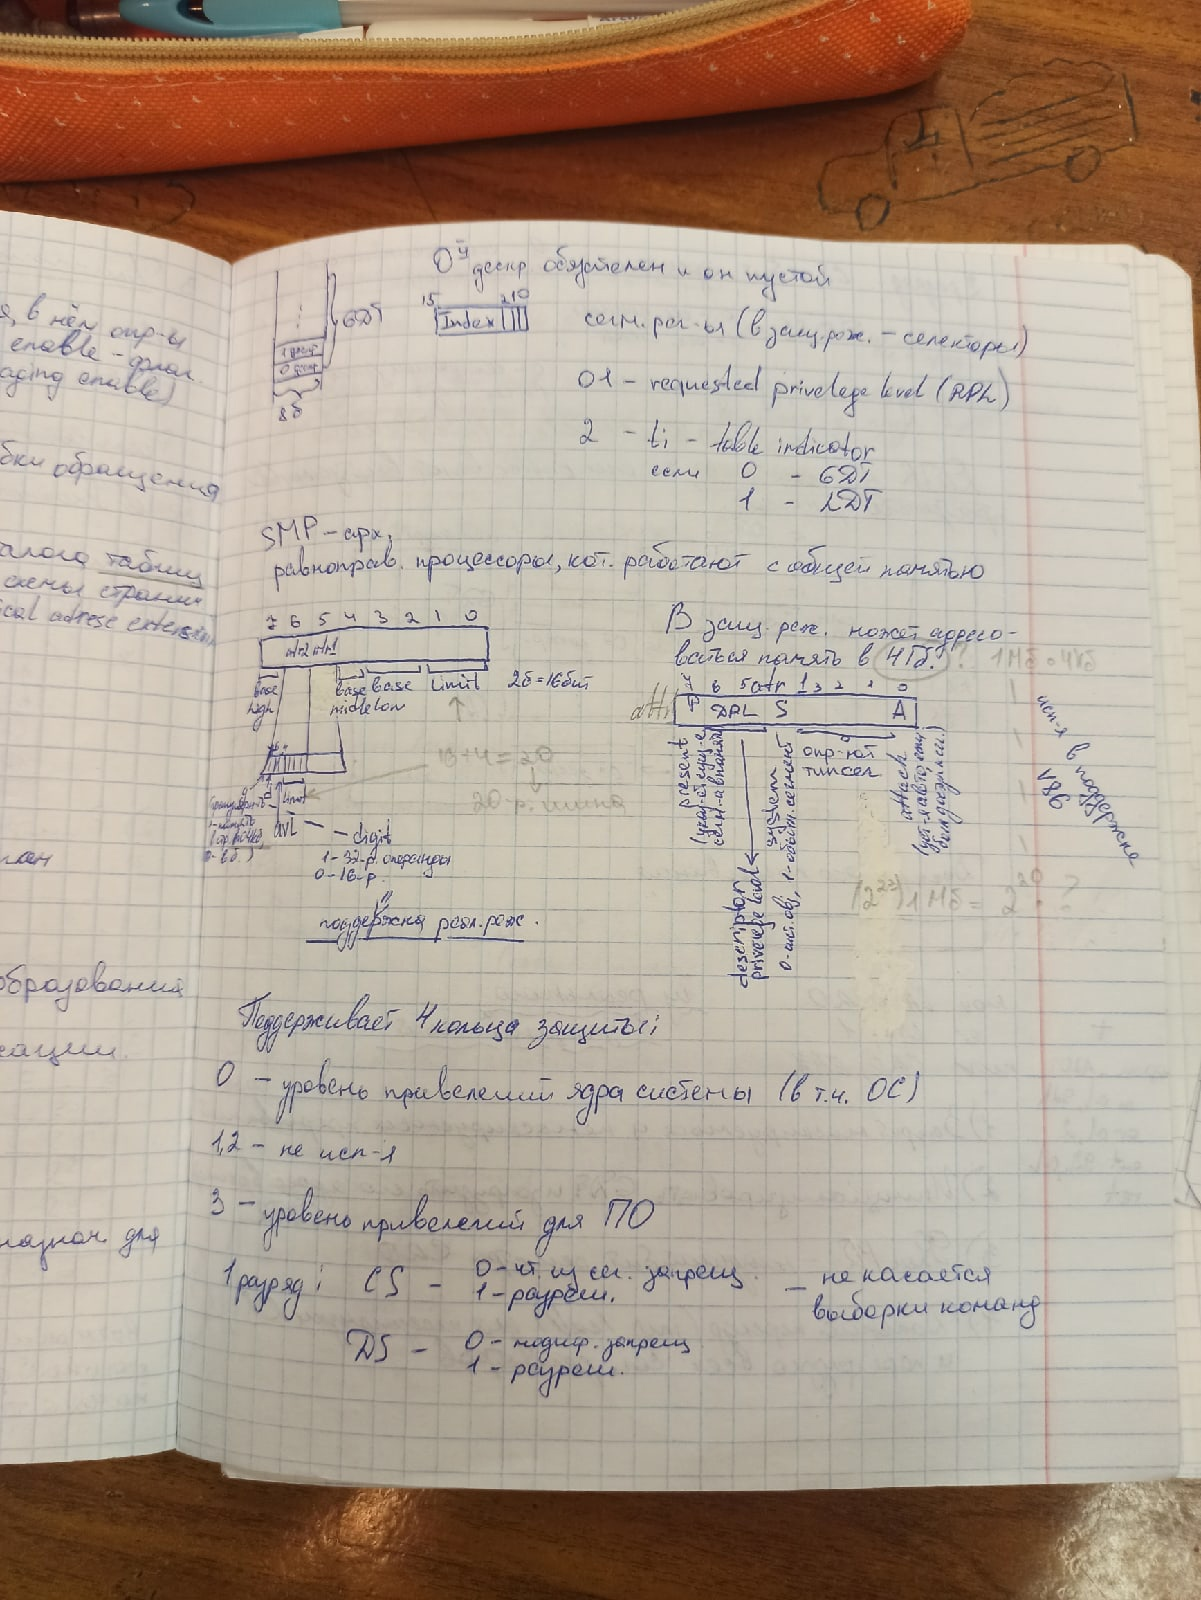
\includegraphics[scale=0.8]{../screens/5.jpg}
	
	""
	
	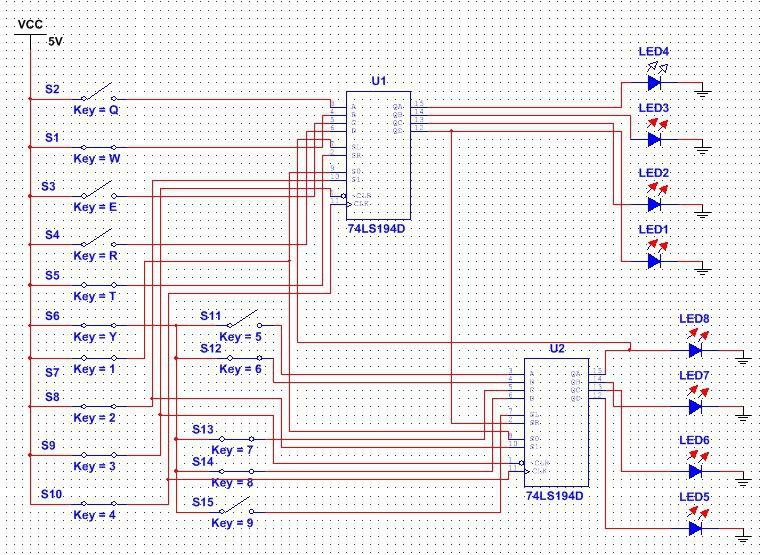
\includegraphics[scale=0.82]{../screens/6.jpg}
\end{center}

\noindent Файл: 3.ms

\section{Наращивание мультиплексора}
Набор значений: 0001 0000 0001 0000
\begin{center}
	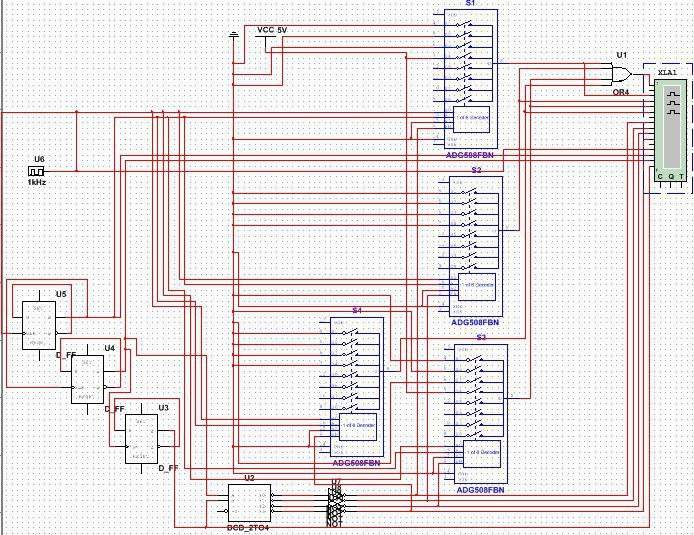
\includegraphics[scale=0.7]{../screens/7.jpg}
	
	""
	
	
\includegraphics[scale=0.73]{../screens/8.jpg}
	
\end{center}

""\newline\newline
\noindent Значения на наращенном мультиплексоре совпадают с исходным, схема работает верно.\newline

\noindent Файл: 4.ms\newline

\section{Вывод}

\noindent При выполнении этой лабораторной работы я изучил принципы построения, практического применения и эксперементально иследовал мультиплексоры.

\section{Контрольные вопросы}

\noindent\textbf{1.} Что такое мультиплексор?\newline

\noindent\textbf{Мультиплексор} -- это функциональный узел, имеющий $n$ адресных входов и $N=^2n$ информационных входов и выполняющий коммутацию на выход того информационного сигнала, адрес (т.е. номер) которого установлен на адресных входах. Мультиплексор переключает сигнал с одной из $N$ входных линий на один выход.
\newline

\noindent\textbf{2.} Какую логическую функцию выполняет мультиплексор? \newline

\noindent
$$ Y = EN \bigvee\limits_{j=0}^{2^n - 1} D_{j} m_{j}(A_{n-1}, A_{n - 2}, ... , A_{i}, ... , A_{1}, A_{0})$$

\noindent $A{i}$ -- адресные входы и сигналы ($i =0, 1, ... n - 1$)

\noindent $D_{j}$ -- информационные входы и сигналы ($j = 0, 1, ..., 2^n-1$)

\noindent $m_{j}$ -- конституента числу, образованному двоичным кодом сигналов на адрессных входах

\noindent $EN$ -- вход и сигнал разрешения (стробирования)\newline

\noindent\textbf{3.} Каково назначение и использование входа разрешения?\newline

\noindent Вход $EN$ используется для:\newline

\noindent -- разрешения работы мультиплексора

\noindent -- стробирования

\noindent -- наращивания числа информационных входов\newline

\noindent При $EN = 1$, разрешается работа мультплексора, при $EN$ -- работа запрещена.\newline

%\clearpage
\noindent\textbf{4.} Какие функции может выполнять мультиплексор?\newline

\noindent Мультиплексоры широко применяются для построения:\newline

\noindent -- коммутаторов-селекторов,

\noindent -- постоянных запоминающих устройств емкостью бит

\noindent -- комбинационных схем, реализующих функции алгебры логики

\noindent -- преобразователей кодов (например, параллельного кода в последовательный) и других узлов.

\clearpage
\noindent\textbf{5.} Какие существуют способы наращивания мультиплексоров?\newline

\noindent Существует два способа наращивания коммутируемых каналов:\newline

\noindent -- по пирамидальной схеме соединения мультиплексоров меньшей размерности

\noindent -- путём выбора мультиплексора группы информационных входов по адресу (т.е. номеру) мультиплексора с помощью дешифратора адреса мультиплексора группы, а затем выбором информационного сигнала мультиплексором группы по адресу информационного сигнала в группе.\newline

\noindent\textbf{6.} Поясните методику синтеза формирователя ФАЛ на мультиплексоре\newline

\noindent Реализация ФАЛ $n$ переменных на мультплексоре с $n$ адресных входами тривиальнa: на адресные входы подаются переменные, на информационные входы -- значения ФАЛ на соответсвующих наборах переменных. На выходе получаем значения ФАЛ в соответсвии с наборами переменных. В этом случае мультплексор -- ПЗУ.\newline

\noindent Для реализации ФАЛ $n + 1$ переменных на адресные входы мультплексора подаются $n$ переменных, на информационных входы $n + 1$-ая переменная (или ее инверсия), константы 0 или 1 (в соответсвии со значениями ФАЛ)\newline

\noindent\textbf{7. } Почему возникают ложные сигналы на выходе мультиплексора? Как их устранить?\newline

\noindent Для исключения на выходе ложных сигналов (их вызывают гонки входных сигналов), вход $EN$ используется как стробирующий. Для выделения полезного сигнала на вход $EN$ подается сигнал в интервале времени, свободном от действия ложных сигналов.
\end{document}